
% ========================================================
% INTRO
% ========================================================
\section{Introduction}\label{s20}
The Compact Pixel Tracking Telescope has two different versions that were both constructed at \ac{ETH} in Zürich. Despite of the name telescope, which literally translated means ``far-seeing'', its main purpose is to detect ionising particles from beam test experiments, i.e. to provide high resolution tracks with pulse heights and precise timing information of the particles that fly through. This information can then be used for other beam test applications such as diamond pad or pixel studies.\\ 
To accomplish that goal it consists of several single \ac{CMS}-Pixel chips that are placed parallel consecutively in a fixed direction which is usually the direction of the beam. The chips are mounted on so-called planes and have a fixed distance to one another that is given by the telescope. The fact of several planes whose appearance resembles objects of an optical device and that it is able to gather information about subatomic particles have given rise to call it a telescope.\\
The data channels of the planes are daisy chained and are accessed by a device called ``test board'' which then sends the data via a USB connection to a computer where it is processed by software. The software that is used now is called ``pXar'' and was written to handle digital chips.
% ========================================================
% 1
% ========================================================
\section{Telescope Layout}\label{s21}
As already mentioned above, there are two versions of the telescope. Version I was designed to be as simple as possible and consists of six planes with analogue chips whereas the second version that was built on the experience with first one, comprises three plane modules (either digital or analogue). The single modules may be combined to bigger modules. Version II has some additional features as well that will be mentioned in the following.\\
Both consist mainly of three parts: a motherboard, adapter planes and the chips.
% ========================================================
\subsection{Motherboard}\label{s210}
The motherboard is the main frame of the telescope. Its printed circuit board (PCB) has a male connector for a parallel data transfer cable to communicate with a test board, which serves as input and once the data is collected as output as well. In case of version II there is a second male connector to which another telescope may be connected that can be used only as an output of the data stream. Next in line after the input come several daisy chained female connectors to plug in the adapter planes. The planes have to be plugged in to the telescope to pass the data, which is collected by a so-called ``token'', to the next plane or, in case of the last plane, to the output. If the telescope is run with less than the maximum amount of planes one can put in a jumper at the vacant position to achieve an unbroken data stream. In addition version I has a LEMO connector that allows to bias all of the connected sensors and version II has a single differential LEMO outputs for a certain signal from the chip called ``fast-OR''. All signals that pass through the telescope are properly terminated by resistors on top the board. In case of version II there are boards with and without resistors and one should take care that only the last board in the chain is one with termination. Otherwise the signals might get too low to be measured.\\
The main differences of the two versions are stated in \ar{t1}.\\
The old telescope was limited to a maximum of six static analogue planes. A main advantage of the new one is its flexibility to chain multiple three-plane telescopes together. %TODO include pic
Furthermore the easiest way to pass the token through an unused plane spot was to hot-wire the correspondent wires of a spare ATA connector and place it instead of the plane (\ar{p2}). With the new telescope you can choose between two jumpers to either pass the token the next plane or loop it in the current one (\ar{p3}). The Dimensions of the telescopes are shown in \ar{p4}.
\begin{figure}[t]
	\begin{minipage}{6cm}
		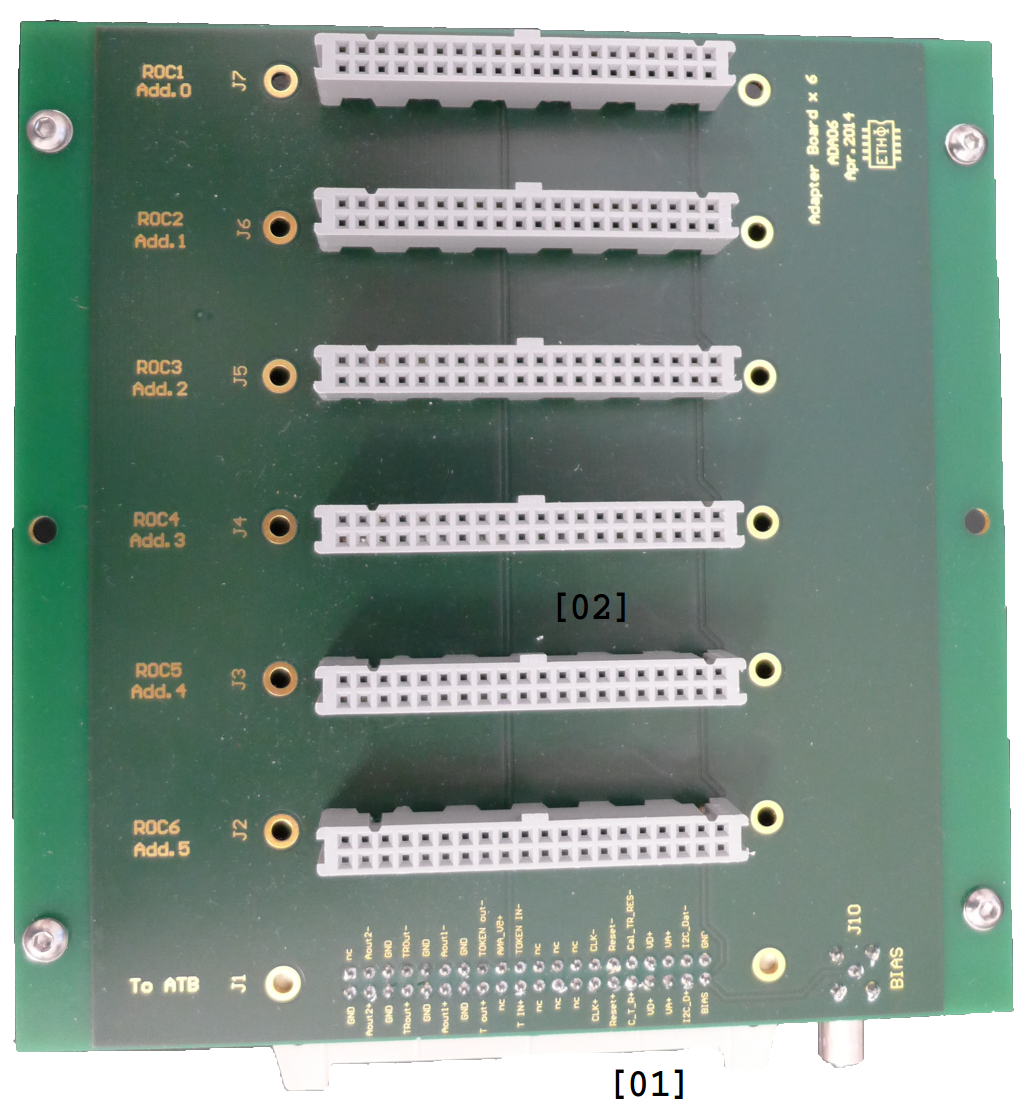
\includegraphics[width=6cm]{Telescope}
		\caption{Telescope version I}
		\label{p0}
	\end{minipage}
	\hfill
	\begin{minipage}{6cm}
		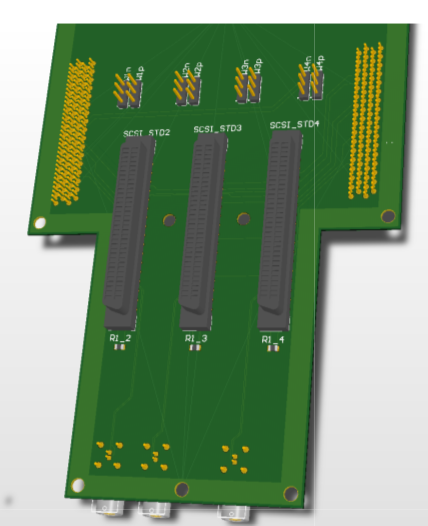
\includegraphics[width=6cm]{Telescope3DTop}
% 			TODO PICTURE OF NEW TELEscope
		\caption{Telescope version II}
		\label{p1}
	\end{minipage}
\end{figure}
\begin{table}[ht]
	\centering
	\begin{tabular}{p{4cm}|c|c}
										& Version I 			& Version II 					\\\hline\hline
		Connector type 					& ATA 40 pin 			& VHDCI 68 pin					\\\hline			
		Number of planes per telescope 	& $6$ 					& $3$							\\\hline
		Maximum number of Planes per read out chain		& $6$					& $3\times3$ \footnotemark[1] \\\hline
		Fast-OR							& directly on the plane	& on the motherboard			\\\hline
		Token jumper					& self made				& next to the connector	\\\hline
		HV connection from the test board	&  constant			& hot-wired by jumper
	\end{tabular}					
	\caption{Differences between the two motherboard versions}
	\label{t1}
\end{table}\no
\footnotetext[1]{Theoretically one could chain an infinite amount of telescopes. In reality the timing between the planes gets worse the longer the data has to travel.}
\begin{figure}[ht]
	\begin{minipage}{6cm}
		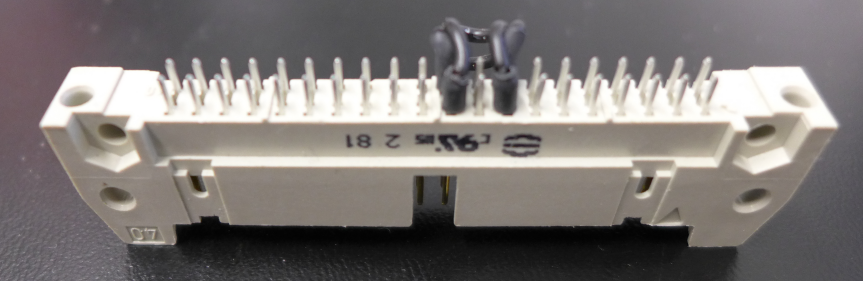
\includegraphics[width=6cm]{TokenJumper}
		\caption{self made token jumper}
		\label{p2}
	\end{minipage}
	\hfill
	\begin{minipage}{6cm}
		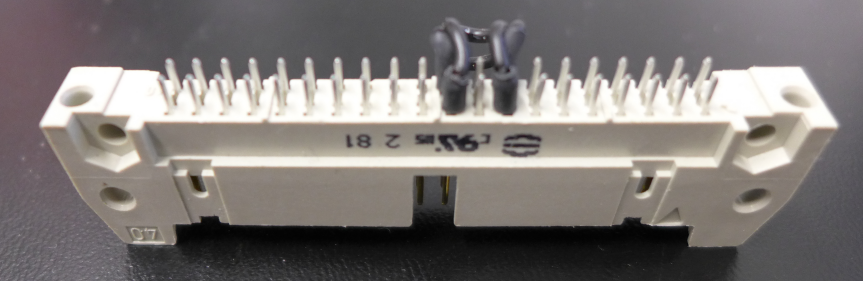
\includegraphics[width=6cm]{TokenJumper}
% 			TODO PICTURE OF NEW Jumper
		\caption{jumper of the new telescope}
		\label{p3}
	\end{minipage}
\end{figure}
% ========================================================
\newpage
\subsection{Adapter Plane}\label{s211}
The adapter plane is the link between the telescope and a single \ac{CMS}-Pixel
\begin{wrapfigure}{r}{6cm}
	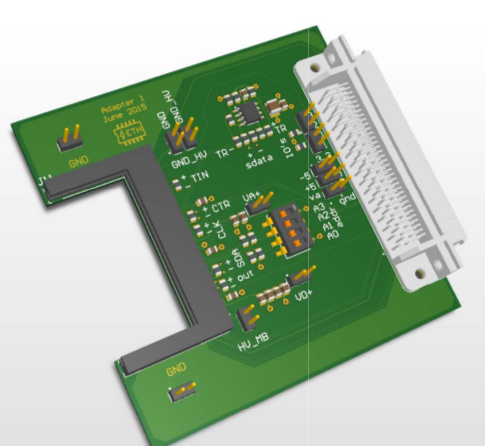
\includegraphics[width=5.9cm]{adapterDig}
	\caption{digital adapter}
	\label{p6}
\end{wrapfigure}
chip. On the bottom end of the PCB is a correspondent male connector by what the plane can be plugged in directly to the motherboard. The analogue planes of the two versions are very similar. The differences are the already mentioned type of  connector and that there are two differential LEMO outputs for the fast-OR on the PCB of version I (\ar{p4}) that were moved to the motherboard in version II (\ar{p5}). Apart from that they both have a LEMO input for biasing the sensor, an amplifying circuit for the signal of the chip and a flat band cable connector to the chip. In version II there is an additional jumper to allow biasing from either the adapter plane or via the connector to the motherboard. In any case, the ground pin of the sensor has to be connected to ground of the SCSI connector with another jumper. In order to bias via the adapter plane a cable has to be connected to a bias pin on the plane, which is linked to the LEMO, and the sensor.\\
The adapter for the digital chips, which is shown in \ar{p6}, can only be used in combination with version II and differs a bit from the analogue one. The only way to bias the digital chips is via the test board and the SCSI connector, which means that there has to be a jumper at ``HV-MB'' and ``GND-HV''. Likewise there are jumpers to connect the supply voltages ``VD'' and `"VA" to the chip. Another very useful improvement is the dip switch box in the middle of the plane, which allows to set a any I2C address between $0$ and $15$. Since the digital chips are put on special PCBs (\ar{p8}) the adapter has a completely different mounting system, s.t. the chips can be easily plugged in and out.
\begin{center}
	\begin{figure}
		\begin{minipage}{6cm}
			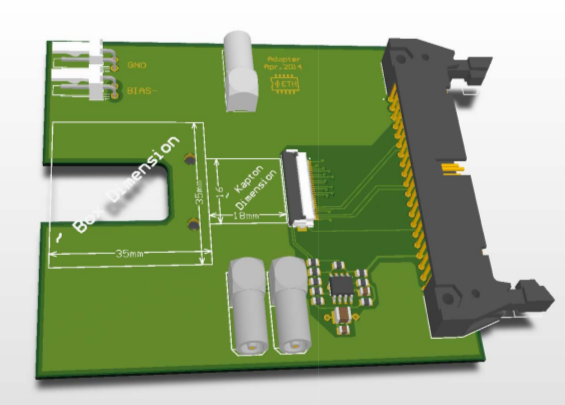
\includegraphics[width=6cm]{adapterAna}
			\caption{analogue adapter I}
			\label{p4}
		\end{minipage}
		\hfill
		\begin{minipage}{6cm}
			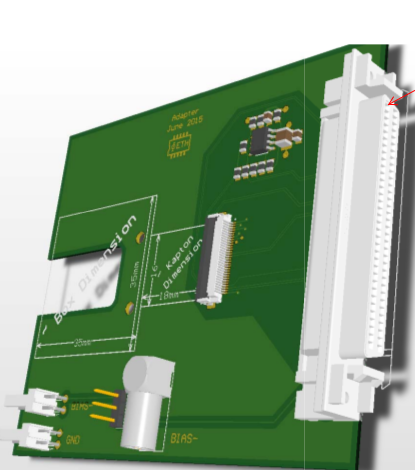
\includegraphics[width=6cm]{adapterAnaII}
% 			TODO PICTURE OF NEW Jumper
			\caption{analogue adapter II}
			\label{p5}
		\end{minipage}
	\end{figure}
\end{center} 

